

Figure \ref{fig:iterations} presents the results of the a cherry picked fair coin
experiment ($\theta_{\rm true}=0.5$). It was chosen to highlight potential stark
different outcomes of the three stop criterion algorithms. For comparison note that the posteriors
shown in Figure \ref{fig:posteriors} are three iterations of this figure.
(TB footnote: 1 - provide the sequence, 2 - reference to JK figure number)

As we can see from both figures at iteration 126 the credible interval (95\% HDI posterior) of HDI+ROPE is fully
outside of the ROPE making it confidently, though incorrectly, reject $\theta_{\rm null}$.The Precision is the Goal stop criterion is met at iteration 598, where the credible
interval width
subpasses the precision goal of 0.08. Since the credible interval straddles the ROPE
the decision is inconclusive.
For the Enhanced Precision is the Goal the credible interval
meets both criterions at iteration 804: narrower than 0.08 precision goal and fully within the ROPE.
This results in correctly accepting $\theta_{\rm null}$.


\begin{figure}[h!]
  \centering
  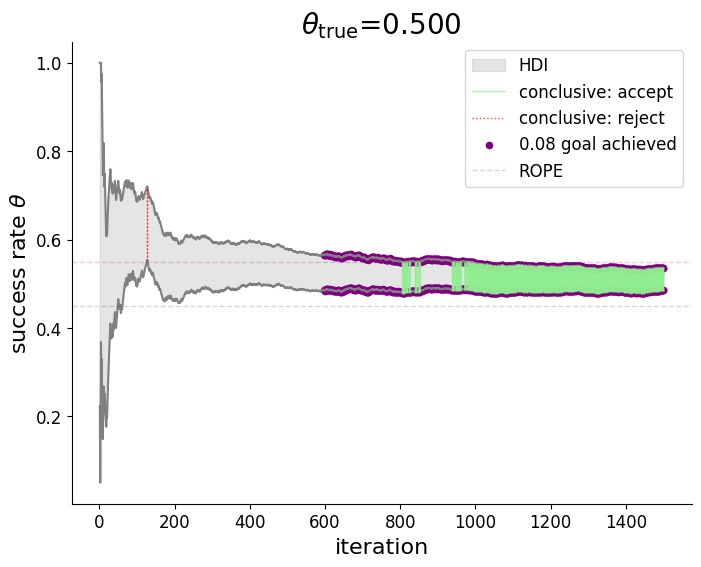
\includegraphics[width=1\textwidth]{cherry_iterations.png}
  \caption{Cherry picked fair coin sample demonstrating the varied outcomes by
  stop criterion mechanism. The vertical axis is the cumulative success rate
  at each iteration (horizontal axis).
  The gray band is the 95\% HDI of the posterior at each iteration.
  The highlighted iterations indicate where stop criterion trigger conditions are met:
  red dashed lines is when  $\theta_{\rm null}$ may be rejected, green solid lines
  is when he $\theta_{\rm null}$ may be accepted. Purple dots on the 95\% HDI boundaries
  indicated when the precision goal is achieved. Note that the posteriors of Figure \ref{fig:posteriors}
  are slices of this figure: HDI+ROPE is the the first red dashed line (iteration 126),
  Precision is the Goal is the first purple dot (598), and Enhanced Precision is the Goal is the second purple dot (598)
  is the first green line (804). The ROPE boundaries is represented by the dashed lines.
  }
  \label{fig:iterations}
\end{figure}

In Figure \ref{fig:fair_iter_vs_rate} we explore how we explore the outcomes of $M=500$
similar experiments and summarise key stats in Table \ref{tab:fair_iter_vs_rate}. (TK Ref JK figure number being additional information to his histograms).


\begin{figure}[h!]
  \centering
  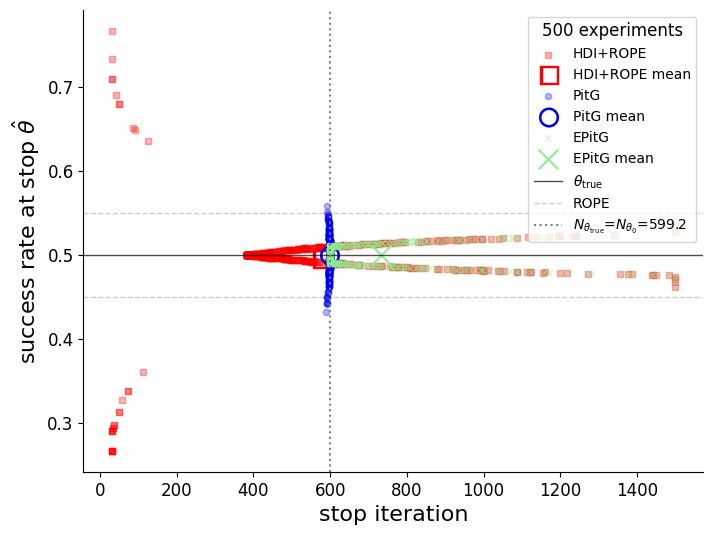
\includegraphics[width=1\textwidth]{fair_experiments_iter_vs_rate.png}
  \caption{Small symbols are individual experiment outcomes. Large are experiments
  mean values. When using HDI+ROPE as the stop criterion results in the red squares.
  Precision is the Goal as the criterion results in the blue circles
  and the Enhanced PitG as the green Xs. $\theta_{\rm true}$ is the solid line and
  the ROPE is the dashed lines. Summary stats are in Table \ref{tab:fair_iter_vs_rate}. TK: analytical results
  }
  \label{fig:fair_iter_vs_rate}
\end{figure}

In the Figure \ref{fig:fair_iter_vs_rate} the large symbols that represent the 500 experiment outcome means 
(large red square, blue circle and X as per legend) show
that on average all methods yield, on average, unbiased outcomes, as per the
$\overline{\theta}$ column in Table \ref{tab:fair_iter_vs_rate}.


\begin{table}[h!]\label{tab:fair_iter_vs_rate}
  \begin{center}
  \begin{tabular}{c|c|c|c|c|c|c|c|c}
    \hline
    Algorithm & Accept & Reject & Conclusive & Inconclusive & $\overline{n}$ & $\sigma_n$ & $\overline{\theta}$ & $\sigma_{\hat{\theta}}$\\
    \hline
    HDI+ROPE & 0.928 & 0.06 & 0.988 & 0.012 & 576.6 & 281 & 0.4952 & 0.0502 \\
    PitG & 0.390 & 0.00 & 0.390 & 0.610 & 598.3 & 1.4 & 0.4994 & 0.01997 \\
    ePitG & 0.984 & 0.00 & 0.984 & 0.016 & 732.2 & 210 & 0.4998 & 0.0127\\
    \hline
  \end{tabular}
  \caption{Stasticsummaries of 500 experiments of three stop criteria shown in Figure \ref{fig:fair_iter_vs_rate}. Accept
  is the fraction of experiments which results in acceptence of $\theta_{\rm null}$,
  and similar for Reject, Conclusive and Inconclusive. Conclusive is the sum of Accept and Reject and Inconclusive is its complementary. The mean stop iteration is $\overline{n}$ and the standard deviation $\sigma_n$
  The mean sample rate at stop is $\overline{\theta}$ and its standard deviation $\sigma_{\hat{\theta}}$.
  }
\end{center}
\end{table}

That said, HDI+ROPE yields falsely accepts $\theta_{\rm null}$ at a rate of 6\% 
whereas the precision methods do not have False Posistives (see Reject column in Table \ref{tab:fair_iter_vs_rate}).
(Note that if we relax the minimum sample size ($N_{\rm min}=0$) the FPR increases to TK\%).
Precision is the Goal (blue circles) stops around iteration ~598 but is 61\% inconclusive.
For conclusiveness of these 61\%, the Enhanced PitG (green Xs) requires more sampling 
resulting in only 1.6\% inconclusive outcomes by final iteration of $N_{\rm max}=1,500$.
This manifests in an average of $732.2\pm 210$ samples per experiment for the Enhanced PitG
compared to $598.3\pm 1.4$ for the Precision is the Goal.

Figure \ref{fig:fair_iter_vs_rate} highlights that after the "Precision stop barrier" at iteration 598 Enhanced Precision is the Goal and HDI+ROPE are the same algorithm.

In Figure \ref{fig:fair_decisions} we explore the decision rates of the three algorithms.
(TK reference to JK's graph).

\begin{figure}[h!]
  \centering
  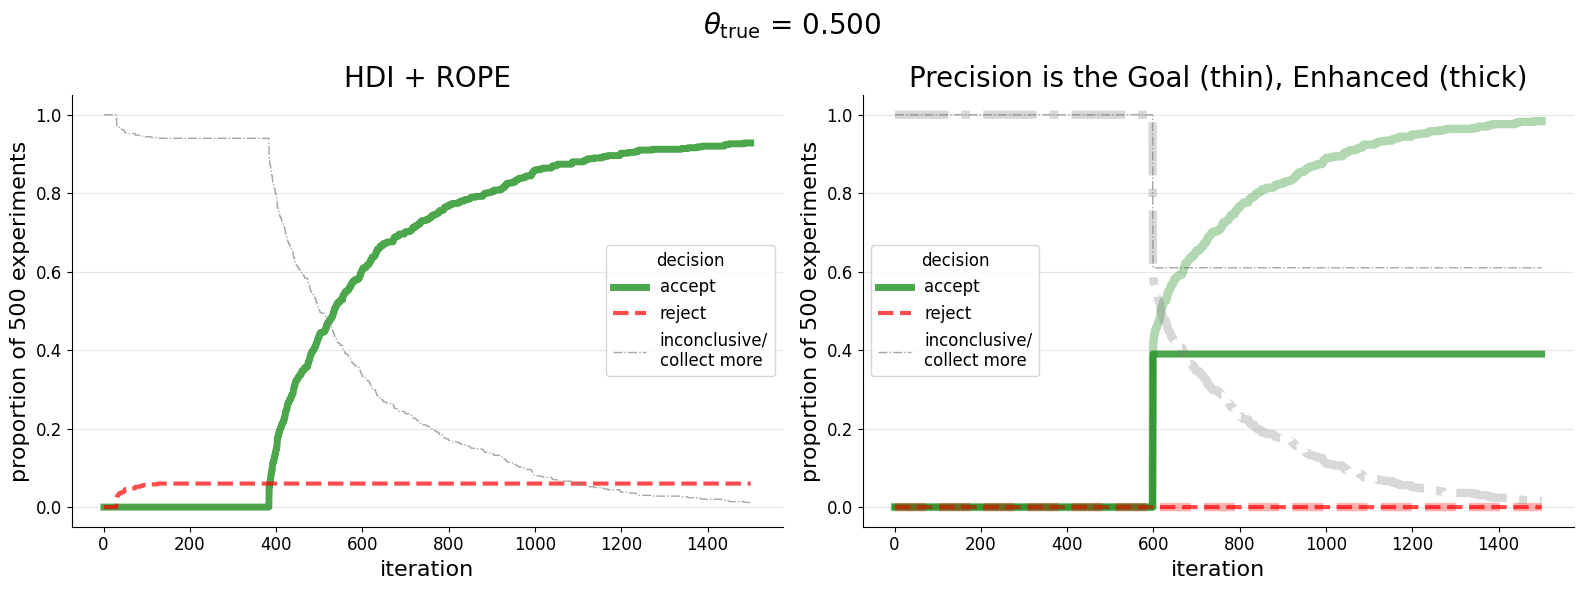
\includegraphics[width=1\textwidth]{fair_experiment_decision_rates.png}
  \caption{Similar information as in Figure \ref{fig:fair_iter_vs_rate} but focusing on the distribution of decisions. Left panel is for HDI+ROPE. Right panel are both precision based methods. Horizontal axis- iteration. Vertical axis- proportion of decisions made up to (and including) each iteration. The sum of Reject (red dashed), Accept (green solid) and Inconclusive/Collect-more- (gray dot-dashed) decisions at each iteration is 100\%.
  }
  \label{fig:fair_decisions}
\end{figure}

We can see that the HDI+ROPE algorithms starts with a high rate of rejection of
$\theta_{\rm null}$ which the precision based methods do not. At around iteration 400
it gradually accepts $\theta_{\rm null}$. In Figure \ref{fig:fair_iter_vs_rate}
this manifests as the red squares being exactly on the $\theta_{\rm true}=0.5$ line
and then gradually moving towards the ROPE boundaries on both sides in a symetric
manner due to the nature of the setup (e.g, we shall see that this symetry
skewes as the coin becomes more loaded). The reason for this is that the mode of
the posteriors deviate slightly from the true value but the credible interval width
is narrow enough to be fully confined within the ROPE.

